\documentclass{ximera}

%\usepackage{todonotes}

\newcommand{\todo}{}

\usepackage{esint} % for \oiint
\ifxake%%https://math.meta.stackexchange.com/questions/9973/how-do-you-render-a-closed-surface-double-integral
\renewcommand{\oiint}{{\large\bigcirc}\kern-1.56em\iint}
\fi


\graphicspath{
  {./}
  {ximeraTutorial/}
  {basicPhilosophy/}
  {functionsOfSeveralVariables/}
  {normalVectors/}
  {lagrangeMultipliers/}
  {vectorFields/}
  {greensTheorem/}
  {shapeOfThingsToCome/}
  {dotProducts/}
  {partialDerivativesAndTheGradientVector/}
  {../productAndQuotientRules/exercises/}
  {../normalVectors/exercisesParametricPlots/}
  {../continuityOfFunctionsOfSeveralVariables/exercises/}
  {../partialDerivativesAndTheGradientVector/exercises/}
  {../directionalDerivativeAndChainRule/exercises/}
  {../commonCoordinates/exercisesCylindricalCoordinates/}
  {../commonCoordinates/exercisesSphericalCoordinates/}
  {../greensTheorem/exercisesCurlAndLineIntegrals/}
  {../greensTheorem/exercisesDivergenceAndLineIntegrals/}
  {../shapeOfThingsToCome/exercisesDivergenceTheorem/}
  {../greensTheorem/}
  {../shapeOfThingsToCome/}
  {../separableDifferentialEquations/exercises/}
  {vectorFields/}
}

\newcommand{\mooculus}{\textsf{\textbf{MOOC}\textnormal{\textsf{ULUS}}}}

\usepackage{tkz-euclide}
\usepackage{tikz}
\usepackage{tikz-cd}
\usetikzlibrary{arrows}
\tikzset{>=stealth,commutative diagrams/.cd,
  arrow style=tikz,diagrams={>=stealth}} %% cool arrow head
\tikzset{shorten <>/.style={ shorten >=#1, shorten <=#1 } } %% allows shorter vectors

\usetikzlibrary{backgrounds} %% for boxes around graphs
\usetikzlibrary{shapes,positioning}  %% Clouds and stars
\usetikzlibrary{matrix} %% for matrix
\usepgfplotslibrary{polar} %% for polar plots
\usepgfplotslibrary{fillbetween} %% to shade area between curves in TikZ
%\usetkzobj{all}
\usepackage[makeroom]{cancel} %% for strike outs
%\usepackage{mathtools} %% for pretty underbrace % Breaks Ximera
%\usepackage{multicol}
\usepackage{pgffor} %% required for integral for loops



%% http://tex.stackexchange.com/questions/66490/drawing-a-tikz-arc-specifying-the-center
%% Draws beach ball
\tikzset{pics/carc/.style args={#1:#2:#3}{code={\draw[pic actions] (#1:#3) arc(#1:#2:#3);}}}



\usepackage{array}
\setlength{\extrarowheight}{+.1cm}
\newdimen\digitwidth
\settowidth\digitwidth{9}
\def\divrule#1#2{
\noalign{\moveright#1\digitwidth
\vbox{\hrule width#2\digitwidth}}}




% \newcommand{\RR}{\mathbb R}
% \newcommand{\R}{\mathbb R}
% \newcommand{\N}{\mathbb N}
% \newcommand{\Z}{\mathbb Z}

\newcommand{\sagemath}{\textsf{SageMath}}


%\renewcommand{\d}{\,d\!}
%\renewcommand{\d}{\mathop{}\!d}
%\newcommand{\dd}[2][]{\frac{\d #1}{\d #2}}
%\newcommand{\pp}[2][]{\frac{\partial #1}{\partial #2}}
% \renewcommand{\l}{\ell}
%\newcommand{\ddx}{\frac{d}{\d x}}

% \newcommand{\zeroOverZero}{\ensuremath{\boldsymbol{\tfrac{0}{0}}}}
%\newcommand{\inftyOverInfty}{\ensuremath{\boldsymbol{\tfrac{\infty}{\infty}}}}
%\newcommand{\zeroOverInfty}{\ensuremath{\boldsymbol{\tfrac{0}{\infty}}}}
%\newcommand{\zeroTimesInfty}{\ensuremath{\small\boldsymbol{0\cdot \infty}}}
%\newcommand{\inftyMinusInfty}{\ensuremath{\small\boldsymbol{\infty - \infty}}}
%\newcommand{\oneToInfty}{\ensuremath{\boldsymbol{1^\infty}}}
%\newcommand{\zeroToZero}{\ensuremath{\boldsymbol{0^0}}}
%\newcommand{\inftyToZero}{\ensuremath{\boldsymbol{\infty^0}}}



% \newcommand{\numOverZero}{\ensuremath{\boldsymbol{\tfrac{\#}{0}}}}
% \newcommand{\dfn}{\textbf}
% \newcommand{\unit}{\,\mathrm}
% \newcommand{\unit}{\mathop{}\!\mathrm}
% \newcommand{\eval}[1]{\bigg[ #1 \bigg]}
% \newcommand{\seq}[1]{\left( #1 \right)}
% \renewcommand{\epsilon}{\varepsilon}
% \renewcommand{\phi}{\varphi}


% \renewcommand{\iff}{\Leftrightarrow}

% \DeclareMathOperator{\arccot}{arccot}
% \DeclareMathOperator{\arcsec}{arcsec}
% \DeclareMathOperator{\arccsc}{arccsc}
% \DeclareMathOperator{\si}{Si}
% \DeclareMathOperator{\scal}{scal}
% \DeclareMathOperator{\sign}{sign}


%% \newcommand{\tightoverset}[2]{% for arrow vec
%%   \mathop{#2}\limits^{\vbox to -.5ex{\kern-0.75ex\hbox{$#1$}\vss}}}
% \newcommand{\arrowvec}[1]{{\overset{\rightharpoonup}{#1}}}
% \renewcommand{\vec}[1]{\arrowvec{\mathbf{#1}}}
% \renewcommand{\vec}[1]{{\overset{\boldsymbol{\rightharpoonup}}{\mathbf{#1}}}}

% \newcommand{\point}[1]{\left(#1\right)} %this allows \vector{ to be changed to \vector{ with a quick find and replace
% \newcommand{\pt}[1]{\mathbf{#1}} %this allows \vec{ to be changed to \vec{ with a quick find and replace
% \newcommand{\Lim}[2]{\lim_{\point{#1} \to \point{#2}}} %Bart, I changed this to point since I want to use it.  It runs through both of the exercise and exerciseE files in limits section, which is why it was in each document to start with.

% \DeclareMathOperator{\proj}{\mathbf{proj}}
% \newcommand{\veci}{{\boldsymbol{\hat{\imath}}}}
% \newcommand{\vecj}{{\boldsymbol{\hat{\jmath}}}}
% \newcommand{\veck}{{\boldsymbol{\hat{k}}}}
% \newcommand{\vecl}{\vec{\boldsymbol{\l}}}
% \newcommand{\uvec}[1]{\mathbf{\hat{#1}}}
% \newcommand{\utan}{\mathbf{\hat{t}}}
% \newcommand{\unormal}{\mathbf{\hat{n}}}
% \newcommand{\ubinormal}{\mathbf{\hat{b}}}

% \newcommand{\dotp}{\bullet}
% \newcommand{\cross}{\boldsymbol\times}
% \newcommand{\grad}{\boldsymbol\nabla}
% \newcommand{\divergence}{\grad\dotp}
% \newcommand{\curl}{\grad\cross}
%\DeclareMathOperator{\divergence}{divergence}
%\DeclareMathOperator{\curl}[1]{\grad\cross #1}
% \newcommand{\lto}{\mathop{\longrightarrow\,}\limits}

% \renewcommand{\bar}{\overline}

\colorlet{textColor}{black}
\colorlet{background}{white}
\colorlet{penColor}{blue!50!black} % Color of a curve in a plot
\colorlet{penColor2}{red!50!black}% Color of a curve in a plot
\colorlet{penColor3}{red!50!blue} % Color of a curve in a plot
\colorlet{penColor4}{green!50!black} % Color of a curve in a plot
\colorlet{penColor5}{orange!80!black} % Color of a curve in a plot
\colorlet{penColor6}{yellow!70!black} % Color of a curve in a plot
\colorlet{fill1}{penColor!20} % Color of fill in a plot
\colorlet{fill2}{penColor2!20} % Color of fill in a plot
\colorlet{fillp}{fill1} % Color of positive area
\colorlet{filln}{penColor2!20} % Color of negative area
\colorlet{fill3}{penColor3!20} % Fill
\colorlet{fill4}{penColor4!20} % Fill
\colorlet{fill5}{penColor5!20} % Fill
\colorlet{gridColor}{gray!50} % Color of grid in a plot

\newcommand{\surfaceColor}{violet}
\newcommand{\surfaceColorTwo}{redyellow}
\newcommand{\sliceColor}{greenyellow}




\pgfmathdeclarefunction{gauss}{2}{% gives gaussian
  \pgfmathparse{1/(#2*sqrt(2*pi))*exp(-((x-#1)^2)/(2*#2^2))}%
}


%%%%%%%%%%%%%
%% Vectors
%%%%%%%%%%%%%

%% Simple horiz vectors
\renewcommand{\vector}[1]{\left\langle #1\right\rangle}


%% %% Complex Horiz Vectors with angle brackets
%% \makeatletter
%% \renewcommand{\vector}[2][ , ]{\left\langle%
%%   \def\nextitem{\def\nextitem{#1}}%
%%   \@for \el:=#2\do{\nextitem\el}\right\rangle%
%% }
%% \makeatother

%% %% Vertical Vectors
%% \def\vector#1{\begin{bmatrix}\vecListA#1,,\end{bmatrix}}
%% \def\vecListA#1,{\if,#1,\else #1\cr \expandafter \vecListA \fi}

%%%%%%%%%%%%%
%% End of vectors
%%%%%%%%%%%%%

%\newcommand{\fullwidth}{}
%\newcommand{\normalwidth}{}



%% makes a snazzy t-chart for evaluating functions
%\newenvironment{tchart}{\rowcolors{2}{}{background!90!textColor}\array}{\endarray}

%%This is to help with formatting on future title pages.
\newenvironment{sectionOutcomes}{}{}



%% Flowchart stuff
%\tikzstyle{startstop} = [rectangle, rounded corners, minimum width=3cm, minimum height=1cm,text centered, draw=black]
%\tikzstyle{question} = [rectangle, minimum width=3cm, minimum height=1cm, text centered, draw=black]
%\tikzstyle{decision} = [trapezium, trapezium left angle=70, trapezium right angle=110, minimum width=3cm, minimum height=1cm, text centered, draw=black]
%\tikzstyle{question} = [rectangle, rounded corners, minimum width=3cm, minimum height=1cm,text centered, draw=black]
%\tikzstyle{process} = [rectangle, minimum width=3cm, minimum height=1cm, text centered, draw=black]
%\tikzstyle{decision} = [trapezium, trapezium left angle=70, trapezium right angle=110, minimum width=3cm, minimum height=1cm, text centered, draw=black]


\title{Analyzing}

\begin{document}

\begin{abstract}
describe everything
\end{abstract}
\maketitle







$\blacktriangleright$ \textbf{\textcolor{red!80!black}{Reasoning:}} Reasoning is a logical explanation that describes our conclusions, how we arrived at those conclusions, and why we think those conclusions are correct. \\

Analysis is not a list of conclusions. We are not looking for such a list. \\

We are looking for the thought process that arrived at the list of conclusions. \\











\begin{example}

\textbf{\textcolor{purple!85!blue}{Completely analyze}} \\


\[   R(t) = \frac{(t+3)(t+1)}{(t-2)(t-3)} \]

with 

\[   R'(t) = -\frac{9 t^2 -6 t -39}{(t-2)^2 (t-3)^2} \]



$R(t)$ is not a composition. It is a rational function. \\


Here is a quick DESMOS graph.


\begin{center}
\desmos{mgkklcsmqr}{400}{300}
\end{center}


There is something wrong with this graph.  $2$ and $3$ make the denominator $0$, but the numbers in the interval $(2, 3)$ are in the domain.  There should be a piece of the graph there that is not showing up.


Let's evalaute at $2.5$ and see what type of values we are getting. \\

$R(2.5) = -77$


\begin{center}
\desmos{8baq5avdvr}{400}{300}
\end{center}


There is the other part of the graph. \\



From the graph, we are anticipating two singularities, two critical numbers, switching between increasing and decreasing, and end-behavior which is not unbounded. \\







































\textbf{\textcolor{blue!55!black}{$\blacktriangleright$ Domain}} 

$R(t)$ is a rational function.  Its domain is all real numbers except the zeros of the denominator. \\

The domain is $(-\infty, 2) \cup (2,3) \cup (3, \infty)$  \\














\textbf{\textcolor{blue!55!black}{$\blacktriangleright$ Zeros}} 


$R(t)$ is a rational function.  Its zeros are the zeros of the numerator except those that are also zeros of the denominator. \\


The zeros of $R$ are $-3$ and $-1$. \\






\textbf{\textcolor{blue!55!black}{$\blacktriangleright$ Continuity}} 


$R(t)$ is a rational function.  It is continuous. \\


$R$ does have singularities.  We need the behavior around them.   Both $2$ and $3$ are zeros of the denominator and not zeros of the numerator.  This makes them asymptotic singularities. \\


We knw know that $R$ is unbounded as $t$ approaches $2$ and $3$.  We need to figure out the sign. \\


\begin{explanation}


For $\lim\limits_{t \to 2^-}R(t)$,  $t < 2$, which gives

\begin{itemize}
\item $t + 3 > 0$
\item $t + 1 > 0$
\item $t - 2 < 0$
\item $t - 3 < 0$
\end{itemize}


The sign of $R$ is $\frac{pos \cdot pos}{neg \cdot neg} = positive$ \\



\[
\lim\limits_{t \to 2^-}R(t) = \infty
\]






For $\lim\limits_{t \to 2^+}R(t)$,  $t > 2$, which gives

\begin{itemize}
\item $t + 3 > 0$
\item $t + 1 > 0$
\item $t - 2 > 0$
\item $t - 3 < 0$
\end{itemize}


The sign of $R$ is $\frac{pos \cdot pos}{pos \cdot neg} = negative$ \\



\[
\lim\limits_{t \to 2^+}R(t) = -\infty
\]





For $\lim\limits_{t \to 3^-}R(t)$,  $t < 3$, which gives

\begin{itemize}
\item $t + 3 > 0$
\item $t + 1 > 0$
\item $t - 2 > 0$
\item $t - 3 < 0$
\end{itemize}


The sign of $R$ is $\frac{pos \cdot pos}{pos \cdot neg} = negative$ \\



\[
\lim\limits_{t \to 2^-}R(t) = -\infty
\]







For $\lim\limits_{t \to 3^+}R(t)$,  $t > 3$, which gives

\begin{itemize}
\item $t + 3 > 0$
\item $t + 1 > 0$
\item $t - 2 > 0$
\item $t - 3 > 0$
\end{itemize}


The sign of $R$ is $\frac{pos \cdot pos}{pos \cdot pos} = positive$ \\



\[
\lim\limits_{t \to 2^-}R(t) = \infty
\]








\end{explanation}



This agrees with the graph.






\textbf{\textcolor{blue!55!black}{$\blacktriangleright$ End-Behavior}} 

$R(t)$ is a rational function. The degree of the numerator and the degree of the denomiator are equal.  The end-behavior is the quotient is the leading coefficients.



\[  
\lim\limits_{t \to -\infty}R(t) = \frac{1}{1} = 1
\]




\[  
\lim\limits_{t \to \infty}R(t) = \frac{1}{1} = 1
\]











\textbf{\textcolor{blue!55!black}{$\blacktriangleright$ Behavior}} 
\textbf{Rate-of-Change}  
\textbf{Increasing and Decreasing}   



The sign of $R'(t)$ will give us the behavior of $R(t)$. \\

To get the sign of $R'(t)$, we will factor it. \\

The denominator is factored.  The numerator is a quadratic function.  To factor it, we need its zeros, which we can get from the quadratic formula. \\

But, first we might as well factor out $3$ in the numerator. \\







\[   
R'(t) = -\frac{9 t^2 -6 t -39}{(t-2)^2 (t-3)^2} = -\frac{3 (3 t^2 - 2 t - 13)}{(t-2)^2 (t-3)^2}
\]




$3 (3 t^2 - 2 t - 13) = 0$ \\

$3 t^2 - 2 t - 13 = 0$ 



\[
t = \frac{2 \pm \sqrt{(-2)^2 - 4(3)(-13)}}{2(3)} = \frac{2 \pm \sqrt{160}}{6} = \frac{2 \pm 4 \sqrt{10}}{6} = \frac{1 \pm 2 \sqrt{10}}{3}
\]




Two critical numbers: $\frac{1 - 2 \sqrt{10}}{3}$ and $\frac{1 + 2 \sqrt{10}}{3}$ \\




Quick Check:  \\


\[
\frac{1 - 2 \sqrt{10}}{3} \approx -1.774851773
\]


\[
\frac{1 + 2 \sqrt{10}}{3} \approx 2.44151844
\]


These agree with the graph, so we feel like our algebra is correct. \\



We can now factor $R'(t)$ \\








\[   
R'(t) = -\frac{3 \left(x - \left(\frac{1 - 2 \sqrt{10}}{3} \right) \right) \left(x - \left(\frac{1 + 2 \sqrt{10}}{3} \right) \right) }{ (t-2)^2 (t-3)^2 } 
\]


Both $\frac{1 - 2 \sqrt{10}}{3}$ and $\frac{1 - 2 \sqrt{10}}{3}$ have odd multiplicities, so $R'$ will change signs across them. \\




Both $2$ and $3$ have even multiplicities, so $R'$ will not change signs across them. \\



We need the order of $\frac{1 - 2 \sqrt{10}}{3}$, $\frac{1 - 2 \sqrt{10}}{3}$, $2$, and $3$.   \\



\begin{explanation}

That graph makes us think that 

\[
\frac{1 - 2 \sqrt{10}}{3} < 2 < \frac{1 + 2 \sqrt{10}}{3} < 3
\]


Let's show that $\frac{1 - 2 \sqrt{10}}{3} < 2$. \\

This true because $\frac{1 - 2 \sqrt{10}}{3} < 0$, since $1 < 2 \sqrt{10}$. \\



Next, we'll show that $2 < \frac{1 + 2 \sqrt{10}}{3}$. \\



This is true if $6 < 1 + 2 \sqrt{10}$, which is true since $3 < \sqrt{10}$. \\



Finally, we need to show that $\frac{1 + 2 \sqrt{10}}{3} < 3$ \\


This is true if $1 + 2 \sqrt{10} < 9$, which is true since $\sqrt{10} < 4$.





\end{explanation}




We now know the ordering of the critical numbers and singularities. \\


\[
\frac{1 - 2 \sqrt{10}}{3} < 2 < \frac{1 + 2 \sqrt{10}}{3} < 3
\]





On $(-\infty, 2)$, 



\[   
R'(t) = -\frac{3 \left(x - \left(\frac{1 - 2 \sqrt{10}}{3} \right) \right) \left(x - \left(\frac{1 + 2 \sqrt{10}}{3} \right) \right) }{ (t-2)^2 (t-3)^2 }  = 
\]






































\textbf{\textcolor{blue!55!black}{$\blacktriangleright$ Extrema}} 


As a strictly increasing function on $(-\infty, \infty)$, $L$ cannot have global or local maximums or minimums. \\










\textbf{\textcolor{blue!55!black}{$\blacktriangleright$ Range}} 



$L$ is a continuous function, never negative, and increasing. In addition, we nkow that 





\[  
\lim\limits_{x \to -\infty}L(x) = \lim\limits_{y \to \infty}f(y) = \lim\limits_{y \to \infty}\frac{5}{1 + 3 y} = 0
\]




\[  
\lim\limits_{x \to \infty}L(x) = \lim\limits_{y \to 0}f(y) = \frac{5}{1 + 3 (0)} = 5
\]








The range of $L$ is $(0, 5)$.













\textbf{\textcolor{blue!55!black}{$\blacktriangleright$ A Graph}} 





The end-behavior tells us that the graph has horizontal asymptotes.










\begin{image}
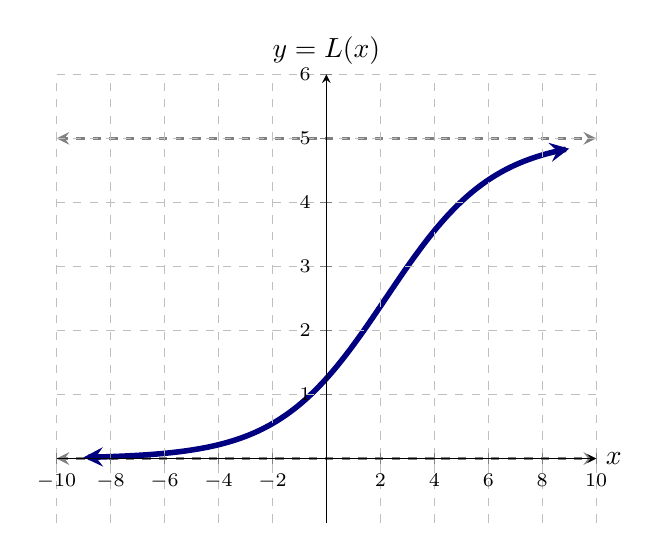
\begin{tikzpicture}
  \begin{axis}[
            domain=-10:10, ymax=6, xmax=10, ymin=-1, xmin=-10,
            axis lines =center, xlabel=$x$, ylabel={$y=L(x)$}, grid = major, grid style={dashed},
            ytick={1,2,3,4,5,6},
            xtick={-10,-8,-6,-4,-2,2,4,6,8,10},
            yticklabels={$1$,$2$,$3$,$4$,$5$,$6$}, 
            xticklabels={$-10$,$-8$,$-6$,$-4$,$-2$,$2$,$4$,$6$,$8$,$10$},
            ticklabel style={font=\scriptsize},
            every axis y label/.style={at=(current axis.above origin),anchor=south},
            every axis x label/.style={at=(current axis.right of origin),anchor=west},
            axis on top
          ]
          
          \addplot [line width=1, gray, dashed,samples=100,domain=(-10:10),<->] {5};
          \addplot [line width=1, gray, dashed,samples=100,domain=(-10:10),<->] {0};

            %\addplot [line width=2, penColor, smooth,samples=100,domain=(-9:9)] {5/(1 + 3 * e^(-x/2))};
          \addplot [line width=2, penColor, smooth,samples=100,domain=(-9:9),<->] {5/(1 + 3 * 2.7182^(-x/2))};

           




           

  \end{axis}
\end{tikzpicture}
\end{image}




\end{example}





\subsection*{with Calculus}

\textbf{\textcolor{red!70!black}{A Peek Ahead...}}




Calculus will give us a formula for the derivative.

\[  L'(x) =   \frac{-15}{2} \cdot \frac{e^{-\tfrac{x}{2}}}{\left(1+3 e^{-\tfrac{x}{2}}\right)^2}    \]


This derivative has no zeros, which tells us that $L(x)$ has no critical numbers.  $L'(x)$ is always positive, which tells us that $L(x)$ is always increasing.












\begin{center}
\textbf{\textcolor{green!50!black}{ooooo-=-=-=-ooOoo-=-=-=-ooooo}} \\

more examples can be found by following this link\\ \link[More Examples of Analyzing Functions]{https://ximera.osu.edu/csccmathematics/precalculus2/precalculus2/analyzingFunctions/examples/exampleList}

\end{center}








\end{document}
